\documentclass[../TDM3_courbe_app.tex]{subfiles}%

\begin{document}
\section[s]"2"{Glissade d'un pingouin sur un igloo}
\enonce{%
	\noindent
	\begin{minipage}{0.70\linewidth}
		Un pingouin, assimilable à un point matériel M de masse $m$ décide de faire
		du toboggan. Il s'élance sans vitesse initiale du sommet A d'un igloo
		voisin, assimilable à une demi sphère $S$ de rayon $R$ et de centre O, posée
		sur un plan horizontal $\Pi$. On considère que le glissement s'effectue sans
		frottement dans le plan vertical ($x$O$z$).
	\end{minipage}
	\hfill
	\begin{minipage}{0.25\linewidth}
		\begin{center}
			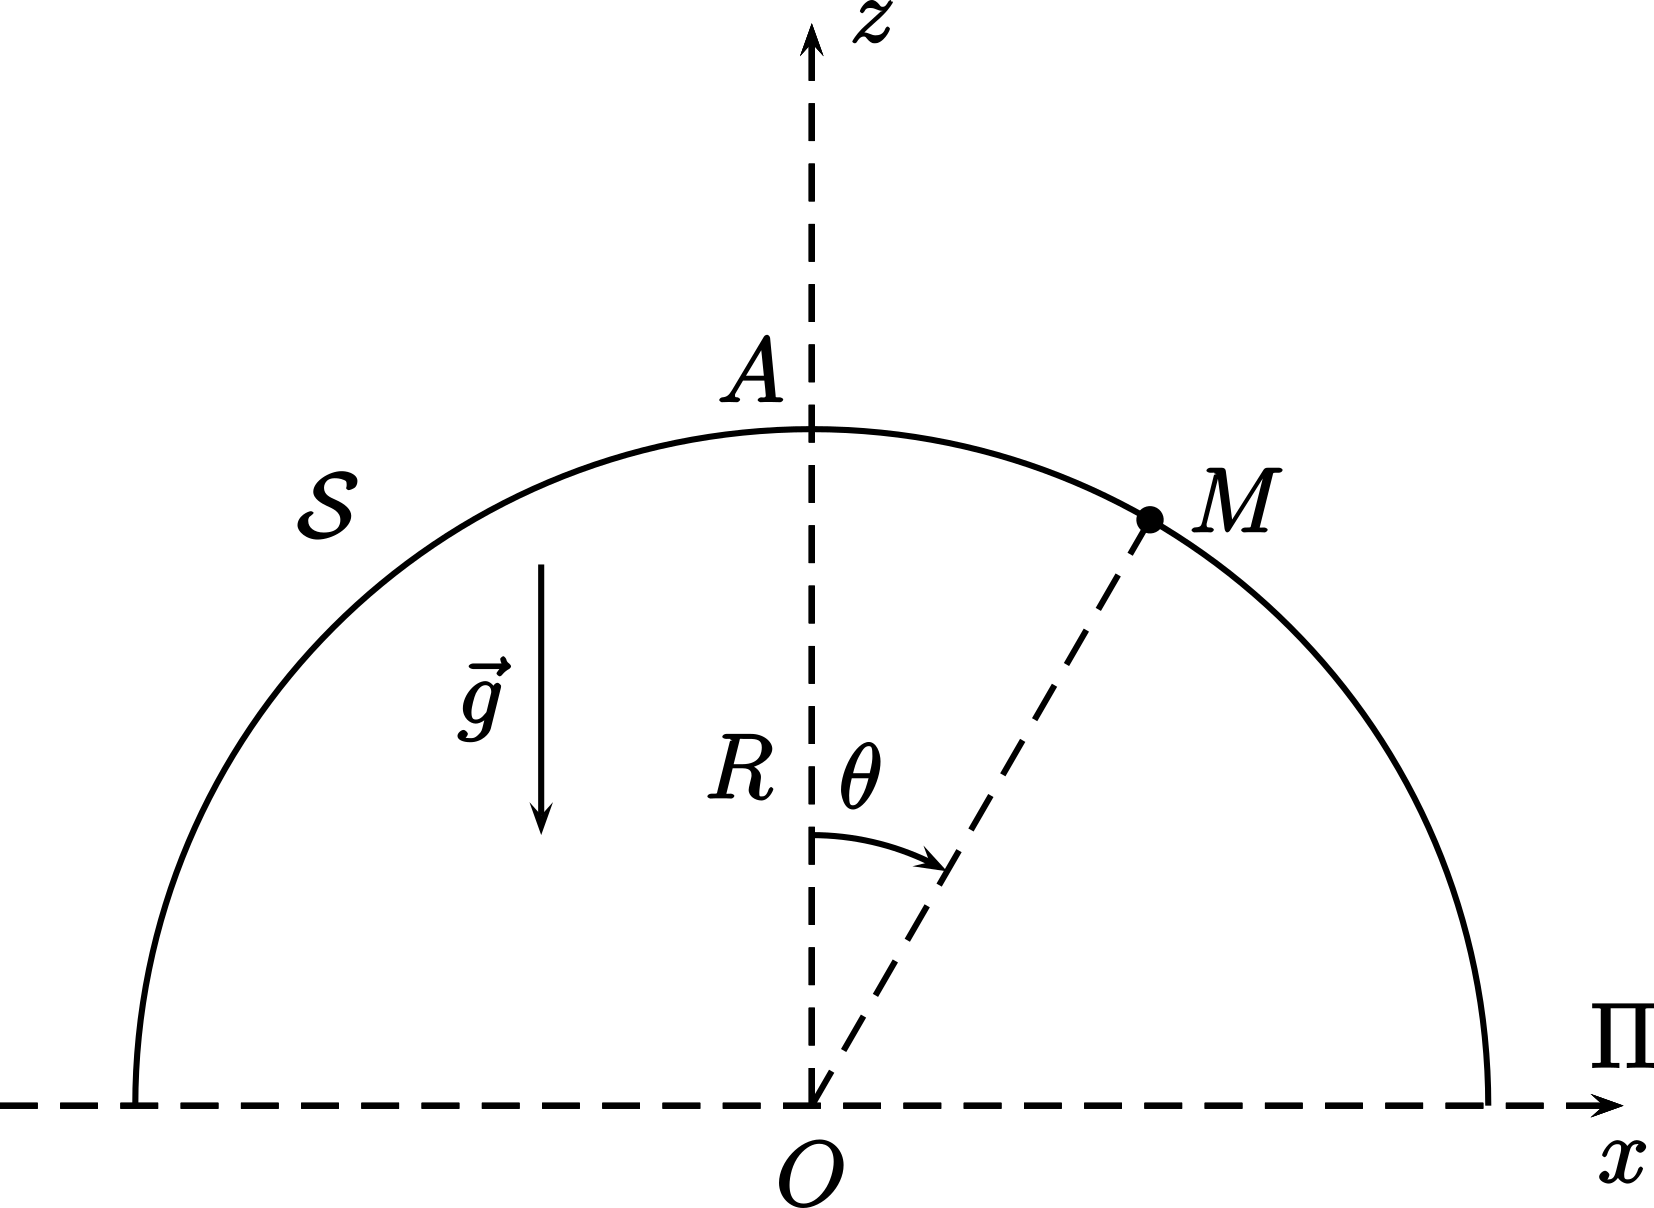
\includegraphics[width=\linewidth]{igloo-plain}
		\end{center}
	\end{minipage}
}

\QR{%
	Appliquer le PFD au pingouin pour en déduire deux équations
	différentielles portant sur l'angle $\th$. Identifier l'équation du
	mouvement qui permet de déterminer $\th(t)$. Quelle information l'autre
	information contient-elle~?
}{%
  \leavevmode\vspace*{-25pt}\relax
	\begin{itemize}[label=$\diamond$, leftmargin=10pt]
		\item[b]{Système}~: \{pingouin\}
	\end{itemize}
	\begin{minipage}{0.70\linewidth}
		\begin{itemize}[label=$\diamond$, leftmargin=10pt]
			\item[b]{Référentiel}~: $\Rc\ind{sol}$ supposé galiléen
			\item[b]{Repère}~: $(\Or, \ur, \ut)$ avec $\ut$ \textbf{dans le sens de
				$\th$}
			\item[b]{Repérage}~:
			\vspace*{-12pt}
			\begin{align*}
				\OM(t) & = R\ur                 \\
				\vf(t) & = R\tp\ut              \\
				\af(t) & = R\tpp\ut - R\tp^2\ur
			\end{align*}
		\end{itemize}
	\end{minipage}
	\hfill
	\begin{minipage}{0.25\linewidth}
		\begin{center}
			\hspace*{-3cm}
			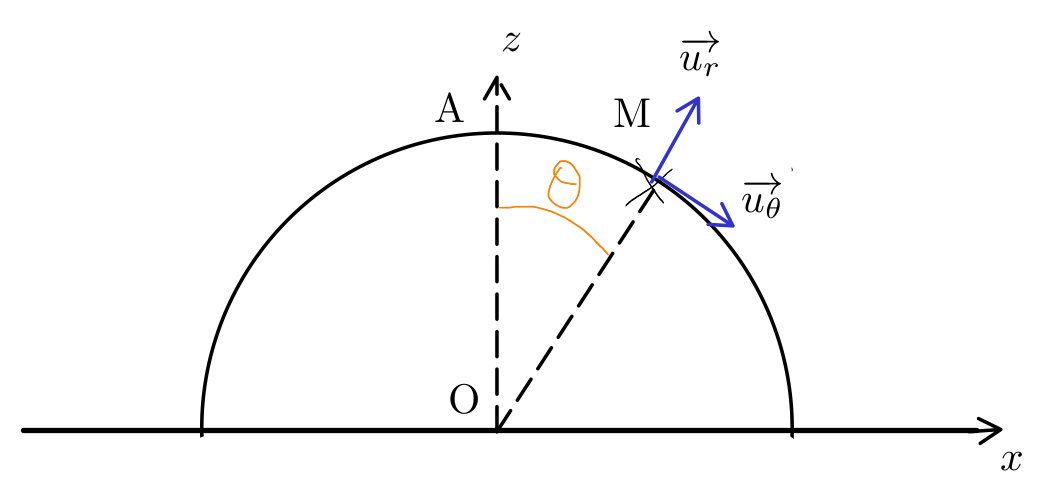
\includegraphics[width=1.8\linewidth]{igloo_corr}
		\end{center}
	\end{minipage}
	\vspace*{12pt}
	\begin{itemize}[label=$\diamond$, leftmargin=10pt]
		\item[b]{Origine et instant initial}~:
		\begin{gather*}
			\OM(0) = \vv{\rm OA} \Ra \th(0) = 0\\
			\vf(0) = \of \Ra \tp(0) = 0
		\end{gather*}
		\item[b]{BDF}~:
		\[
			\begin{array}{ll}
				\textbf{Poids}    & \Pf = mg(-\cos\th\ur +\sin\th\ut) \\
				\textbf{Réaction} & \Rf = R_N\ur
			\end{array}
		\]
		\item \leftcenters{\textbf{PFD}~:}{
			      $\DS
				      m\af = \Pf + \Rf
				      \Lra
				      \mqty(-mR\tp^2\\mR\tpp) = \mqty(-mg\cos\th+R_N\\mg\sin\th)
			      $}
		      \begin{empheq}[box=\fbox, left=\Lra\empheqlbrace]{align}
			      \label{eq:pinga}
			      R_N  & = mg\cos\th - mR\tp^2\\
			      \label{eq:pingb}
			      \tpp & = \frac{g}{R}\sin\th
		      \end{empheq}
	\end{itemize}
	L'équation du mouvement est celle qui donne l'équation d'oscillateur
	harmonique aux petits angles, et qu'on a déjà utilisée en cours sur le
	pendule, et linéaire en $\th$~: l'équation~\eqref{eq:pingb}.
	L'équation~\eqref{eq:pinga} contient l'information sur le contact à
	l'igloo.
}
\QR{%
	En multipliant l'équation du mouvement par $\tp$ et en intégrant sur
	$t$, montrer que
	\[\tp^2 = \frac{2g}{R}(1-\cos\th)\]
}{%
	En prenant~\eqref{eq:pingb}$\times\tp$, on a
	\begin{align*}
		\tpp\tp
		              & = \frac{g}{R} \tp\sin\th
		\\\Lra
		\dv{t}(\frac{1}{2}\tp^2)
		              & = \frac{g}{R} \dv{t}(-\cos\th)
		\\\Lra
		\frac{1}{2}\int_{t=0}^{t} \dv{\tp^2}{t}\dt
		              & = \frac{g}{R}\int_{t=0}^{t} \dv{(-\cos\th)}{t}\dt
		\\\Lra
		\frac{1}{2} \left[ \tp^2 \right]_{t=0}^{t}
		              & = \frac{g}{R} \left[ -\cos\th \right]_{t=0}^{t}
		\\\Lra
		\Aboxed{\tp^2 & = \frac{2g}{R}(1-\cos\th)}
		\qed
	\end{align*}
}
\QR{%
	En déduire la norme de la force de réaction de l'igloo.
}{%
	En reprenant~\eqref{eq:pinga}, on peut remplacer $\tp^2$~:
	\begin{align*}
		R_N         & = mg\cos\th -m\cancel{R}\frac{2g}{\cancel{R}}(1-\cos\th)
		\\\Lra
		\Aboxed{R_N & = mg(3\cos\th -2)}
	\end{align*}
}
\QR{%
	Le pingouin décolle-t-il du toit de l'igloo avant d'atteindre le sol~?
	Si oui, pour quel angle~?
}{%
	La condition de support d'un solide est $R_N > 0$~: le pingouin
	décolle du support si la force de réaction est nulle, soit $R_N = 0$.
	Or,
	\begin{align*}
		R_N          & = 0
		\\\Lra
		3\cos\th - 2 & =0
		\\\Lra
		\Aboxed{\th  & = \arccos(\frac{2}{3})}
	\end{align*}
	Une application numérique donne \fbox{$\th = \ang{48.2}$}.
}

\end{document}
